\documentclass[UTF8,a4paper,12pt]{ctexbook} 

\usepackage{graphicx}%学习插入图
\usepackage{verbatim}%学习注释多行
\usepackage{booktabs}%表格
\usepackage{geometry}%图片
\usepackage{amsmath}
\usepackage{amssymb}
\usepackage{listings}%代码
\usepackage{xcolor}  %颜色
\usepackage{enumitem}%列表格式
\setenumerate[1]{itemsep=0pt,partopsep=0pt,parsep=\parskip,topsep=5pt}
\setitemize[1]{itemsep=0pt,partopsep=0pt,parsep=\parskip,topsep=5pt}
\setdescription{itemsep=0pt,partopsep=0pt,parsep=\parskip,topsep=5pt}
\usepackage{tcolorbox}
\usepackage{algorithm}  %format of the algorithm
\usepackage{algorithmic}%format of the algorithm
\usepackage{multirow}   %multirow for format of table
\usepackage{tabularx} 	%表格排版格式控制
\usepackage{array}	%表格排版格式控制
\usepackage{hyperref} %超链接 \url{URL}
\usepackage{tikz}
\usepackage{dirtree}


\usetikzlibrary{intersections,
	positioning,
	petri,
	backgrounds,
	fit,
	decorations.pathmorphing,
	arrows,
	arrows.meta,
	bending,
	calc,
	intersections,
	through,
	backgrounds,
	shapes.geometric,
	quotes,
	matrix,
	trees,
	shapes.symbols,
	graphs,
	math,
	patterns,
	external}
\CTEXsetup[format+={\flushleft}]{section}

%%%% 设置图片目录
\setmainfont{Times New Roman}
\graphicspath{{figure/}}

%%%% 段落首行缩进两个字 %%%%
\makeatletter
\let\@afterindentfalse\@afterindenttrue
\@afterindenttrue
\makeatother
\setlength{\parindent}{2em}  %中文缩进两个汉字位

%%%% 下面的命令重定义页面边距,使其符合中文刊物习惯 %%%%
\addtolength{\topmargin}{-54pt}
\setlength{\oddsidemargin}{0.63cm}  % 3.17cm - 1 inch
\setlength{\evensidemargin}{\oddsidemargin}
\setlength{\textwidth}{14.66cm}
\setlength{\textheight}{24.00cm}    % 24.62

%%%% 下面的命令设置行间距与段落间距 %%%%
\linespread{1.4}
\setlength{\parskip}{0.5\baselineskip}
\geometry{left=1.6cm,right=1.8cm,top=2cm,bottom=1.7cm} %设置文章宽度
\pagestyle{plain} 		  %设置页面布局

%代码效果定义
\definecolor{mygreen}{rgb}{0,0.6,0}
\definecolor{mygray}{rgb}{0.5,0.5,0.5}
\definecolor{mymauve}{rgb}{0.58,0,0.82}
\lstset{ %
	backgroundcolor=\color{white},   % choose the background color
	basicstyle=\footnotesize\ttfamily,      % size of fonts used for the code
	%stringstyle=\color{codepurple},
	%basicstyle=\footnotesize,
	%breakatwhitespace=false,         
	%breaklines=true,                 
	%captionpos=b,                    
	%keepspaces=true,                 
	%numbers=left,                    
	%numbersep=5pt,                  
	%showspaces=false,                
	%showstringspaces=false,
	%showtabs=false,        
	columns=fullflexible,
	breaklines=true,                 % automatic line breaking only at whitespace
	captionpos=b,                    % sets the caption-position to bottom
	tabsize=4,
	commentstyle=\color{mygreen},    % comment style
	escapeinside={\%*}{*)},          % if you want to add LaTeX within your code
	keywordstyle=\color{blue},       % keyword style
	stringstyle=\color{mymauve}\ttfamily,     % string literal style
	frame=single,
	rulesepcolor=\color{red!20!green!20!blue!20},
	% identifierstyle=\color{red},
	language=c++,
}
 \author{\kaishu 郑华}
 \title{\heiti 数据结构笔记}
 
\begin{document}          %正文排版开始
 	\maketitle
 	\tableofcontents
 	
\chapter{链表}


\chapter{堆}


\chapter{栈}


\chapter{树}
	\section{二叉树前序、中序、后序遍历相互求法}
		首先,我们看看前序、中序、后序遍历的特性: 
		
		前序遍历: 
		\begin{enumerate}[itemindent = 2em]
			\item 访问根节点 
			\item 前序遍历左子树 
			\item 前序遍历右子树
		\end{enumerate}
		
		中序遍历: 
		\begin{enumerate}[itemindent = 2em]
			\item 前序遍历左子树 
			\item 访问根节点 
			\item 前序遍历右子树
		\end{enumerate}
		
		后序遍历: 
		\begin{enumerate}[itemindent = 2em]
			\item 前序遍历左子树 
			\item 前序遍历右子树
			\item 访问根节点 
		\end{enumerate}
		
		\subparagraph{一、已知前序、中序遍历,求后序遍历}:
		
			前序遍历:         GDAFEMHZ
			
			中序遍历:         ADEFGHMZ
			
			\begin{enumerate}[itemindent = 1em]
				\item 根据前序遍历的特点,我们知道根结点为G根据前序遍历的特点,我们知道根结点为G
				\item 观察中序遍历ADEFGHMZ。其中root节点G左侧的ADEF必然是root的左子树,G右侧的HMZ必然是root的右子树
				\item 观察左子树ADEF,左子树的中的根节点必然是大树的root的leftchild。在前序遍历中,大树的root的leftchild位于root之后,所以左子树的根节点为D
				\item 同样的道理,root的右子树节点HMZ中的根节点也可以通过前序遍历求得。在前序遍历中,一定是先把root和root的所有左子树节点遍历完之后才会遍历右子树,并且遍历的左子树的第一个节点就是左子树的根节点。同理,遍历的右子树的第一个节点就是右子树的根节点。
				\item 观察发现,上面的过程是递归的
			\end{enumerate}
		
		\subparagraph{二、已知中序和后序遍历,求前序遍历}:
		
			\begin{enumerate}[itemindent = 1em]
				\item 根据后序遍历的特点,我们知道后序遍历最后一个结点即为根结点,即根结点为G。
				\item 观察中序遍历ADEFGHMZ。其中root节点G左侧的ADEF必然是root的左子树,G右侧的HMZ必然是root的右子树。
				\item 观察左子树ADEF,左子树的中的根节点必然是大树的root的leftchild。在前序遍历中,大树的root的leftchild位于root之后,所以左子树的根节点为D。
				\item 同样的道理,root的右子树节点HMZ中的根节点也可以通过前序遍历求得。在前后序遍历中,一定是先把root和root的所有左子树节点遍历完之后才会遍历右子树,并且遍历的左子树的第一个节点就是左子树的根节点。同理,遍历的右子树的第一个节点就是右子树的根节点。
				\item 观察发现,上面的过程是递归的
			\end{enumerate}
		
		\subparagraph{三、总结}
			根据上述思路,则大体思想如下:
			
			\begin{enumerate}[itemindent = 1em]
				\item 确定根,确定左子树,确定右子树。
				\item 在左子树中递归。
				\item 在右子树中递归。
				\item 打印当前根。
			\end{enumerate}
			
			结果如图\ref{mid_first}所示:
				\begin{figure}
					\centering
					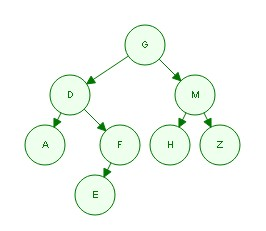
\includegraphics[scale = 1]{Tree_Mid_First.jpg}
					\caption{根据先序和中序确定二叉树}
					\label{mid_first}
				\end{figure}
		
		\subparagraph{四、代码实现思路}


	\section{平衡二叉树}
		我们知道,对于一般的二叉搜索树(Binary Search Tree),其期望高度(即为一棵平衡树时)为log2n,其各操作的时间复杂度O(log2n)同时也由此而决定。但是,在某些极端的情况下(如在插入的序列是有序的时),二叉搜索树将退化成近似链或链,此时,其操作的时间复杂度将退化成线性的,即O(n)。我们可以通过随机化建立二叉搜索树来尽量的避免这种情况,但是在进行了多次的操作之后,由于在删除时,我们总是选择将待删除节点的后继代替它本身,这样就会造成总是右边的节点数目减少,以至于树向左偏沉。这同时也会造成树的平衡性受到破坏,提高它的操作的时间复杂度。于是就有了我们下边介绍的平衡二叉树。
		
		平衡二叉树定义:平衡二叉树(Balanced Binary Tree)又被称为AVL树(有别于AVL算法),且具有以下性质:它是一 棵空树或\textbf{它的左右两个子树的高度差的绝对值不超过1,并且左右两个子树都是一棵平衡二叉树}。平衡二叉树的常用算法有红黑树、AVL树等。在平衡二叉搜索树中,我们可以看到,\textbf{其高度一般都良好地维持在O(log2n),大大降低了操作的时间复杂度}。
		
		最小二叉平衡树的节点的公式如下:
		
		F(n)=F(n-1)+F(n-2)+1
		
		这个类似于一个递归的数列,可以参考Fibonacci数列,1是根节点,F(n-1)是左子树的节点数量,F(n-2)是右子树的节点数量。
			\begin{lstlisting}[frame = L, xleftmargin = .07\textwidth]
	// 求树高度
	int high(btnode *T)  
	{  
		if(T==NULL)  
			return 0;  
		else  
			return max(high(T->lchild),high(T->rchild))+1;  
	}  
	
	
	// 方法2
	void high(bnode *T,int &h)    引用h为树的高度  
	{  
		if(T==NULL)  
			h=0;  
		else  
		{  
			int h1,h2;  
			high(T->lchild,h1);  
			high(T->rchild,h2);  
			h=max(h1,h2)+1;  
		}  
	}  
			\end{lstlisting}
			
			\subsection{平衡查找树之AVL树}
				AVL树定义:AVL树是最先发明的自平衡二叉查找树。在AVL中任何节点的两个儿子子树的高度最大差别为1,所以它也被称为高度平衡树,n个结点的AVL树最大深度约1.44log2n。查找、插入和删除在平均和最坏情况下都是O(logn)。增加和删除可能需要通过一次或多次树旋转来重新平衡这个树。这个方案很好的解决了二叉查找树退化成链表的问题,把插入,查找,删除的时间复杂度最好情况和最坏情况都维持在O(logN)。但是频繁旋转会使插入和删除牺牲掉O(logN)左右的时间,不过相对二叉查找树来说,时间上稳定了很多。
				
				AVL树的自平衡操作——旋转:
				
				AVL树最关键的也是最难的一步操作就是旋转。旋转主要是为了实现AVL树在实施了插入和删除操作以后,树重新回到平衡的方法。下面我们重点研究一下AVL树的旋转。
				
				对于一个平衡的节点,由于任意节点最多有两个儿子,因此高度不平衡时,此节点的两颗子树的高度差2.容易看出,这种不平衡出现在下面四种情况:
				\begin{figure}[H]
					\centering
					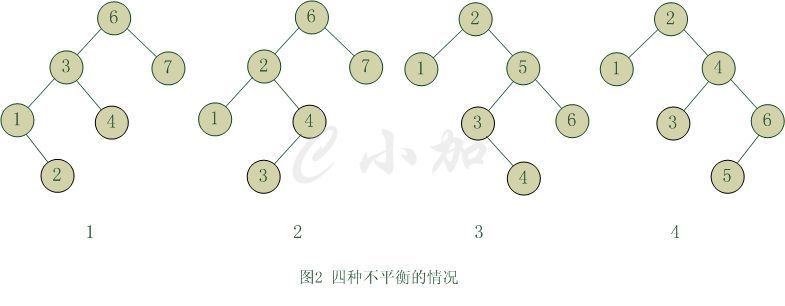
\includegraphics[scale = 0.8]{AVL.jpg}
					\caption{AVL 4种不平衡}
					\label{AVL}
				\end{figure}
					
				\begin{enumerate}[itemindent = 1em,label = (\arabic{enumi})]
					\item  6节点的左子树3节点高度比右子树7节点大2,左子树3节点的左子树1节点高度大于右子树4节点,这种情况成为左左。
					\item  6节点的左子树2节点高度比右子树7节点大2,左子树2节点的左子树1节点高度小于右子树4节点,这种情况成为左右。
					\item  2节点的左子树1节点高度比右子树5节点小2,右子树5节点的左子树3节点高度大于右子树6节点,这种情况成为右左。
					\item  2节点的左子树1节点高度比右子树4节点小2,右子树4节点的左子树3节点高度小于右子树6节点,这种情况成为右右。
				\end{enumerate}
				
				从图\ref{AVL}中可以可以看出,1和4两种情况是对称的,这两种情况的旋转算法是一致的,只需要经过一次旋转就可以达到目标,我们称之为单旋转。2和3两种情况也是对称的,这两种情况的旋转算法也是一致的,需要进行两次旋转,我们称之为双旋转。
					
				\subparagraph{单旋转}:
				
					单旋转是针对于\textbf{左左}和\textbf{右右}这两种情况的解决方案,这两种情况是对称的,只要解决了左左这种情况,右右就很好办了。图3是左左情况的解决方案,节点k2不满足平衡特性,因为它的左子树k1比右子树Z深2层,而且k1子树中,更深的一层的是k1的左子树X子树,所以属于左左情况。
						\begin{figure}[H]
							\centering
							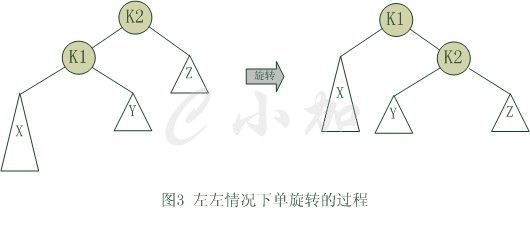
\includegraphics[scale = 0.8]{Rotate_1.jpg}
							\caption{AVL 单旋转}
						\end{figure}
						
					为使树恢复平衡,我们把k2变成这棵树的根节点,因为k2大于k1,把k2置于k1的右子树上,而原本在k1右子树的Y大于k1,小于k2,就把Y置于k2的左子树上,这样既满足了二叉查找树的性质,又满足了平衡二叉树的性质。
					
					这样的操作只需要一部分指针改变,结果我们得到另外一颗二叉查找树,它是一棵AVL树,因为X向上一移动了一层,Y还停留在原来的层面上,Z向下移动了一层。整棵树的新高度和之前没有在左子树上插入的高度相同,插入操作使得X高度长高了。因此,由于这颗子树高度没有变化,所以通往根节点的路径就不需要继续旋转了。
						
				\subparagraph{双旋转}:
				
					对于\textbf{左右}和\textbf{右左}这两种情况,单旋转不能使它达到一个平衡状态,要经过两次旋转。双旋转是针对于这两种情况的解决方案,同样的,这样两种情况也是对称的,只要解决了左右这种情况,右左就很好办了。图4是左右情况的解决方案,节点k3不满足平衡特性,因为它的左子树k1比右子树Z深2层,而且k1子树中,更深的一层的是k1的右子树k2子树,所以属于左右情况。
					\begin{figure}[H]
						\centering
						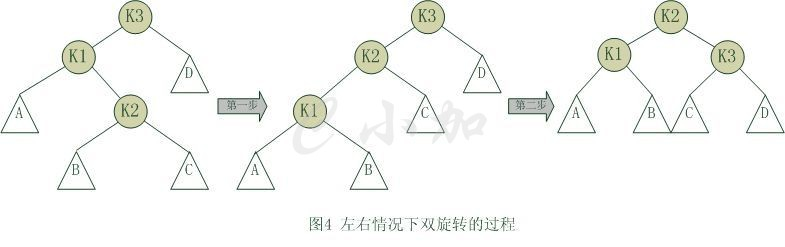
\includegraphics[scale = 0.8]{Rotate_2.jpg}
						\caption{AVL 双旋转}
					\end{figure}
					
					为使树恢复平衡,我们需要进行两步,第一步,把k1作为根,进行一次右右旋转,旋转之后就变成了左左情况,所以第二步再进行一次左左旋转,最后得到了一棵以k2为根的平衡二叉树。
				
				\subparagraph{实现}:
					\begin{lstlisting}[frame = lines]
	//AVL树节点信息
	template<class T>
	class TreeNode
	{
	public:
		TreeNode():lson(NULL),rson(NULL),freq(1),hgt(0){}
		T data;//值
		int hgt;//高度
		unsigned int freq;//频率
		TreeNode* lson;//指向左儿子的地址
		TreeNode* rson;//指向右儿子的地址
	};
	
	//AVL树类的属性和方法声明
	template<class T>
	class AVLTree
	{
	private:
		TreeNode<T>* root;//根节点
		void insertpri(TreeNode<T>* &node,T x);//插入
		TreeNode<T>* findpri(TreeNode<T>* node,T x);//查找
		void insubtree(TreeNode<T>* node);//中序遍历
		void Deletepri(TreeNode<T>* &node,T x);//删除
		int height(TreeNode<T>* node);//求树的高度
		void SingRotateLeft(TreeNode<T>* &k2);//左左情况下的旋转
		void SingRotateRight(TreeNode<T>* &k2);//右右情况下的旋转
		void DoubleRotateLR(TreeNode<T>* &k3);//左右情况下的旋转
		void DoubleRotateRL(TreeNode<T>* &k3);//右左情况下的旋转
		int Max(int cmpa,int cmpb);//求最大值
	
	public:
		AVLTree():root(NULL){}
		void insert(T x);//插入接口
		TreeNode<T>* find(T x);//查找接口
		void Delete(T x);//删除接口
		void traversal();//遍历接口
	
	};
	//计算节点的高度
	template<class T>
	int AVLTree<T>::height(TreeNode<T>* node)
	{
		if(node!=NULL)
			return node->hgt;
		return -1;
	}
	//求最大值
	template<class T>
	int AVLTree<T>::Max(int cmpa,int cmpb)
	{
		return cmpa>cmpb?cmpa:cmpb;
	}
	//左左情况下的旋转
	template<class T>
	void AVLTree<T>::SingRotateLeft(TreeNode<T>* &k2)
	{
		TreeNode<T>* k1;
		k1=k2->lson;
		k2->lson=k1->rson;
		k1->rson=k2;
		
		k2->hgt=Max(height(k2->lson),height(k2->rson))+1;
		k1->hgt=Max(height(k1->lson),k2->hgt)+1;
	}
	//右右情况下的旋转
	template<class T>
	void AVLTree<T>::SingRotateRight(TreeNode<T>* &k2)
	{
		TreeNode<T>* k1;
		k1=k2->rson;
		k2->rson=k1->lson;
		k1->lson=k2;
		
		k2->hgt=Max(height(k2->lson),height(k2->rson))+1;
		k1->hgt=Max(height(k1->rson),k2->hgt)+1;
	}
	//左右情况的旋转
	template<class T>
	void AVLTree<T>::DoubleRotateLR(TreeNode<T>* &k3)
	{
		SingRotateRight(k3->lson);
		SingRotateLeft(k3);
	}
	//右左情况的旋转
	template<class T>
	void AVLTree<T>::DoubleRotateRL(TreeNode<T>* &k3)
	{
		SingRotateLeft(k3->rson);
		SingRotateRight(k3);
	}
	//插入
	template<class T>
	void AVLTree<T>::insertpri(TreeNode<T>* &node,T x)
	{
		if(node==NULL)//如果节点为空,就在此节点处加入x信息
		{
			node=new TreeNode<T>();
			node->data=x;
			return;
		}
		if(node->data>x)//如果x小于节点的值,就继续在节点的左子树中插入x
		{
			insertpri(node->lson,x);
			if(2==height(node->lson)-height(node->rson))
				if(x<node->lson->data)
					SingRotateLeft(node);
				else
					DoubleRotateLR(node);
		}
		else if(node->data<x)//如果x大于节点的值,就继续在节点的右子树中插入x
		{
			insertpri(node->rson,x);
			if(2==height(node->rson)-height(node->lson))//如果高度之差为2的话就失去了平衡,需要旋转
				if(x>node->rson->data)
					SingRotateRight(node);
				else
					DoubleRotateRL(node);
		}
		else ++(node->freq);//如果相等,就把频率加1
		node->hgt=Max(height(node->lson),height(node->rson));
	}
	//插入接口
	template<class T>
	void AVLTree<T>::insert(T x)
	{
		insertpri(root,x);
	}
	//查找
	template<class T>
	TreeNode<T>* AVLTree<T>::findpri(TreeNode<T>* node,T x)
	{
		if(node==NULL)//如果节点为空说明没找到,返回NULL
		{
			return NULL;
		}
		if(node->data>x)//如果x小于节点的值,就继续在节点的左子树中查找x
		{
			return findpri(node->lson,x);
		}
		else if(node->data<x)//如果x大于节点的值,就继续在节点的左子树中查找x
		{
			return findpri(node->rson,x);
		}
		else return node;//如果相等,就找到了此节点
	}
	//查找接口
	template<class T>
	TreeNode<T>* AVLTree<T>::find(T x)
	{
		return findpri(root,x);
	}
	//删除
	template<class T>
	void AVLTree<T>::Deletepri(TreeNode<T>* &node,T x)
	{
		if(node==NULL) return ;//没有找到值是x的节点
		if(x < node->data)
		{
			Deletepri(node->lson,x);//如果x小于节点的值,就继续在节点的左子树中删除x
			if(2==height(node->rson)-height(node->lson))
				if(node->rson->lson!=NULL&&(height(node->rson->lson)>height(node->rson->rson)) )
					DoubleRotateRL(node);
				else
					SingRotateRight(node);
		}
		
		else if(x > node->data)
		{
			Deletepri(node->rson,x);//如果x大于节点的值,就继续在节点的右子树中删除x
			if(2==height(node->lson)-height(node->rson))
				if(node->lson->rson!=NULL&& (height(node->lson->rson)>height(node->lson->lson) ))
					DoubleRotateLR(node);
				else
					SingRotateLeft(node);
		}
		
		else//如果相等,此节点就是要删除的节点
		{
			if(node->lson&&node->rson)//此节点有两个儿子
			{
				TreeNode<T>* temp=node->rson;//temp指向节点的右儿子
				while(temp->lson!=NULL) temp=temp->lson;//找到右子树中值最小的节点
				//把右子树中最小节点的值赋值给本节点
				node->data=temp->data;
				node->freq=temp->freq;
				Deletepri(node->rson,temp->data);//删除右子树中最小值的节点
				if(2==height(node->lson)-height(node->rson))
				{
					if(node->lson->rson!=NULL&& (height(node->lson->rson)>height(node->lson->lson) ))
					DoubleRotateLR(node);
					else
					SingRotateLeft(node);
				}
			}
			else//此节点有1个或0个儿子
			{
				TreeNode<T>* temp=node;
				if(node->lson==NULL)//有右儿子或者没有儿子
					node=node->rson;
				else if(node->rson==NULL)//有左儿子
					node=node->lson;
				delete(temp);
				temp=NULL;
			}
		}
		
		if(node==NULL) return;
		node->hgt=Max(height(node->lson),height(node->rson))+1;
		return;
	}
	//删除接口
	template<class T>
	void AVLTree<T>::Delete(T x)
	{
		Deletepri(root,x);
	}
	//中序遍历函数
	template<class T>
	void AVLTree<T>::insubtree(TreeNode<T>* node)
	{
		if(node==NULL) return;
		insubtree(node->lson);//先遍历左子树
		cout<<node->data<<" ";//输出根节点
		insubtree(node->rson);//再遍历右子树
	}
	//中序遍历接口
	template<class T>
	void AVLTree<T>::traversal()
	{
		insubtree(root);
	}
				\end{lstlisting}
				
				
			\subsection{平衡查找树之红黑树}
				红黑树的\textbf{定义}:红黑树是一种自平衡二叉查找树,是在计算机科学中用到的一种数据结构,典型的用途是实现关联数组。它是在1972年由鲁道夫·贝尔发明的,称之为"对称二叉B树",它现代的名字是在 Leo J. Guibas 和 Robert Sedgewick 于1978年写的一篇论文中获得的。它是复杂的,但它的操作有着良好的最坏情况运行时间,并且在实践中是高效的: 它可以在O(logn)时间内做查找,插入和删除,这里的n是树中元素的数目。
				
				红黑树和AVL树一样都对插入时间、删除时间和查找时间提供了最好可能的最坏情况担保。这不只是使它们在时间敏感的应用如实时应用(real time application)中有价值,而且使它们有在提供最坏情况担保的其他数据结构中作为建造板块的价值;例如,在计算几何中使用的很多数据结构都可以基于红黑树。此外,红黑树还是2-3-4树的一种等同,它们的思想是一样的,只不过红黑树是2-3-4树用二叉树的形式表示的。
				
				\subparagraph{红黑树的性质}:
				
					红黑树是每个节点都带有颜色属性的二叉查找树,颜色为红色或黑色。在二叉查找树强制的一般要求以外,对于任何有效的红黑树我们增加了如下的额外要求:
					
					性质1. 节点是红色或黑色。
					
					性质2. 根是黑色。
					
					性质3. 所有叶子都是黑色(叶子是NIL节点)。
					
					性质4. 每个红色节点必须有两个黑色的子节点。(从每个叶子到根的所有路径上不能有两个连续的红色节点。)
					
					性质5. 从任一节点到其每个叶子的所有简单路径都包含相同数目的黑色节点。
			\subsection{B 树}
				B树也是一种用于查找的平衡树,但是它不是二叉树。
				
				B树的定义:B树(B-tree)是一种树状数据结构,能够用来存储排序后的数据。这种数据结构能够让查找数据、循序存取、插入数据及删除的动作,都在对数时间内完成。B树,概括来说是一个一般化的二叉查找树,可以拥有多于2个子节点。与自平衡二叉查找树不同,B-树为系统最优化大块数据的读和写操作。B-tree算法减少定位记录时所经历的中间过程,从而加快存取速度。这种数据结构常被应用在数据库和文件系统的实作上。
				
				在B树中查找给定关键字的方法是,首先把根结点取来,在根结点所包含的关键字K1,…,Kn查找给定的关键字(可用顺序查找或二分查找法),若找到等于给定值的关键字,则查找成功;否则,一定可以确定要查找的关键字在Ki与Ki+1之间,Pi为指向子树根节点的指针,此时取指针Pi所指的结点继续查找,直至找到,或指针Pi为空时查找失败。
				
				\textbf{B树作为一种多路搜索树}(并不是二叉的):
				
				1) 定义任意非叶子结点最多只有M个儿子;且M>2;
				
				2) 根结点的儿子数为[2, M];
				
				3) 除根结点以外的非叶子结点的儿子数为[M/2, M];
				
				4) 每个结点存放至少M/2-1(取上整)和至多M-1个关键字;(至少2个关键字)
				
				5) 非叶子结点的关键字个数=指向儿子的指针个数-1;
				
				6) 非叶子结点的关键字:K[1], K[2], …, K[M-1];且K[i] < K[i+1];
				
				7) 非叶子结点的指针:P[1], P[2], …, P[M];其中P[1]指向关键字小于K[1]的子树,P[M]指向关键字大于K[M-1]的子树,其它P[i]指向关键字属于(K[i-1], K[i])的子树;
				
				8) 所有叶子结点位于同一层;
			
			\subsection{B+ 树}
				B+树是B树的变体,也是一种多路搜索树:
				
				1) 其定义基本与B-树相同,除了:
				
				2) 非叶子结点的子树指针与关键字个数相同;
				
				3) 非叶子结点的子树指针P[i],指向关键字值属于[K[i], K[i+1])的子树(B-树是开区间);
				
				4) 为所有叶子结点增加一个链指针;
				
				5) 所有关键字都在叶子结点出现;
				
			\subsection{B* 树}
				B*树是B+树的变体,在B+树的非根和非叶子结点再增加指向兄弟的指针,将结点的最低利用率从1/2提高到2/3。
			
		\section{Trie 字典树}	
			Tire树称为字典树,又称单词查找树,Trie树,是一种树形结构,是一种哈希树的变种。典型应用是用于统计,排序和保存大量的字符串(但不仅限于字符串),所以经常被搜索引擎系统用于文本词频统计。它的优点是:利用字符串的公共前缀来减少查询时间,最大限度地减少无谓的字符串比较,查询效率比哈希树高。 
			
			\textbf{Tire树的三个基本性质}:
				\begin{enumerate}[itemindent = 1em]
					\item 根节点不包含字符,除根节点外每一个节点都只包含一个字符
					\item 从根节点到某一节点,路径上经过的字符连接起来,为该节点对应的字符串
					\item 每个节点的所有子节点包含的字符都不相同
				\end{enumerate}

			\textbf{Tire树的应用}:

			1) \textbf{串的快速检索}
			
			给出N个单词组成的熟词表,以及一篇全用小写英文书写的文章,请你按最早出现的顺序写出所有不在熟词表中的生词。
			
			在这道题中,我们可以用数组枚举,用哈希,用字典树,先把熟词建一棵树,然后读入文章进行比较,这种方法效率是比较高的。
			
			2) \textbf{“串”排序}
			
			给定N个互不相同的仅由一个单词构成的英文名,让你将他们按字典序从小到大输出。用字典树进行排序,采用数组的方式创建字典树,这棵树的每个结点的所有儿子很显然地按照其字母大小排序。对这棵树进行先序遍历即可。
			
			3) \textbf{最长公共前缀}
			
			对所有串建立字典树,对于两个串的最长公共前缀的长度即他们所在的结点的公共祖先个数,于是,问题就转化为求公共祖先的问题。


\chapter{哈希}


  
		    
\end{document} 
 		    